\documentclass[11pt]{article}
\usepackage{booktabs}
\usepackage{natbib}
\usepackage{fullpage}
\usepackage{fancyhdr}
\usepackage{rotating}

\usepackage{amsmath}
\usepackage{amssymb}
\usepackage{url}

\usepackage{listings}
\usepackage{color}
\lstset{%
        basicstyle=\footnotesize\ttfamily,
        showspaces=false,
        showstringspaces=false,
        tabsize=2,
        breaklines=false,
        breakatwhitespace=true,
        identifierstyle=\ttfamily,
        keywordstyle=\color[rgb]{0,0,1},
        commentstyle=\color[rgb]{0.133,0.545,0.133},
        stringstyle=\color[rgb]{0.627,0.126,0.941},
    }

\usepackage{graphicx}

% header
\fancyhead{}
\fancyfoot{}
\fancyfoot[C]{\thepage}
\fancyhead[R]{Daniel Foreman-Mackey}
\fancyhead[L]{Statistical Natural Language Processing --- Final Project}
\pagestyle{fancy}
\setlength{\headsep}{10pt}
\setlength{\headheight}{20pt}

% shortcuts
\newcommand{\Eq}[1]{Equation (\ref{eq:#1})}
\newcommand{\eq}[1]{Equation (\ref{eq:#1})}
\newcommand{\eqlabel}[1]{\label{eq:#1}}
\newcommand{\Fig}[1]{Figure~\ref{fig:#1}}
\newcommand{\fig}[1]{Figure~\ref{fig:#1}}
\newcommand{\figlabel}[1]{\label{fig:#1}}

\newcommand{\etal}{\emph{et al.}}

\newcommand{\pr}[1]{\ensuremath{p\left (#1 \right )}}
\newcommand{\lk}[1]{\ensuremath{\mathcal{L} \left ( #1 \right )}}
\newcommand{\bvec}[1]{\ensuremath{\boldsymbol{#1}}}
\newcommand{\dd}{\ensuremath{\, \mathrm{d}}}
\newcommand{\normal}[2]{\ensuremath{\mathcal{N} \left ( #1; #2 \right ) }}
\newcommand{\T}{^\mathrm{T}}
\newcommand{\expect}[2]{\ensuremath{\mathrm{E}_{#1}\left [ {#2} \right ]}}

\newcommand{\data}{\mathcal{D}}
\newcommand{\code}[1]{{\sffamily #1}}
\DeclareMathOperator*{\argmax}{arg\,max}


\begin{document}

\section{Variational LDA}

Th basic LDA model is shown in the top panel of \fig{lda}.
In this model, there is a set of $K$ topics that describe $D$ documents with
$N_d$ words (in a vocabulary of $J$ words) each.
The generative procedure is:
\begin{itemize}
\item{for each topic $k=1,\cdots,K$, draw a word distribution
$\beta_k \sim \mathrm{Dirichlet}(\eta)$,}
\item{for each document $d=1,\cdots,D$, draw a topic distribution $\theta_d
\sim \mathrm{Dirichlet}(\alpha)$, and then}
\item{for each word $n=1,\cdots,N_d$, draw a topic
$z_{d,n}\sim\mathrm{Multinomial}(\theta_d)$ and specific word
$w_{d,n}\sim\mathrm{Multinomial}(\beta_{z_{d,n}})$.}
\end{itemize}
To be specific, the relevant distributions are
\begin{eqnarray}
p(\beta_k\,|\,\eta) &=&
\frac{\Gamma\left( \sum_j \eta_j \right)}{\sum_j \Gamma(\eta_j)} \,
\prod_{j=1}^J \beta_{k,j}^{\eta_j-1} \quad, \\
p(\theta_d\,|\,\alpha) &=&
\frac{\Gamma\left( \sum_k \alpha_k \right)}{\sum_k \Gamma(\alpha_k)} \,
\prod_{k=1}^K \theta_{d,k}^{\alpha_k-1} \quad, \\
p(z_{d,n}\,|\,\theta_d) &=& \theta_{d,z_{d,n}} \quad, \\
p(w_{d,n}\,|\,z_{d,n},\beta) &=& \beta_{z_{d,n},w_{d,n}} \quad.
\end{eqnarray}

To do parameter estimation in this model, we need to compute the marginalized
likelihood
\begin{eqnarray}
p(w\,|\,\alpha,\eta) &=& \int\dd\beta\dd\theta\dd z \,
    p(w,z,\theta,\beta\,|\,\alpha,\eta)
\end{eqnarray}
and optimize but this marginalization is intractable so we have to resort to
approximate methods.

\begin{figure}
\begin{center}
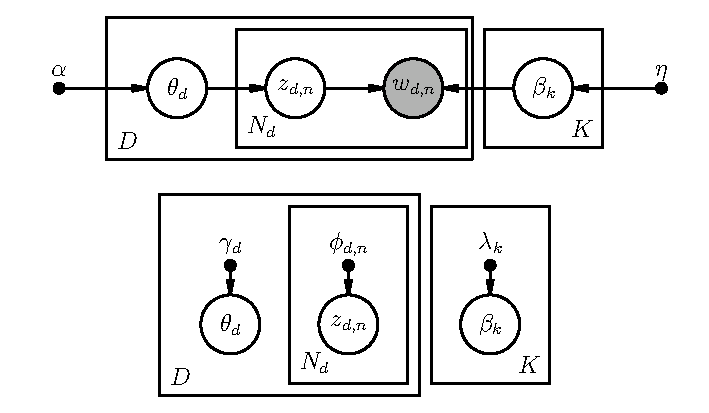
\includegraphics{lda.pdf}
\end{center}
\caption{%
LDA
\figlabel{lda}}
\end{figure}

\subsection{Computing the perplexity}

The marginalized log-likelihood is
\begin{eqnarray}
\log p (\bvec{w}\,|\,\bvec{\alpha},\bvec{\beta}) &\le&
    \expect{q}{\log p
        (\bvec{\theta},\bvec{z},\bvec{w}\,|\,\bvec{\alpha},\bvec{\beta})}
    - \expect{q}{\log q(\bvec{\theta},\bvec{z})} \quad.
\end{eqnarray}
Some useful quantities needed for computing this number are
\begin{eqnarray}
\expect{q}{\log p(\bvec{\theta}\,|\,\bvec{\alpha})} &=&
    \log \Gamma \left ( \sum_k \alpha_k \right )
    - \sum_k \log \Gamma \left ( \alpha_k \right )
    + \sum_k (\alpha_k - 1)\,\expect{q}{\log \theta_k} \\
&=& \log \Gamma \left ( \sum_k \alpha_k \right )
    - \sum_k \log \Gamma \left ( \alpha_k \right )
    + \sum_k (\alpha_k - 1)\,
    \left [ \Psi (\gamma_k) - \Psi \left(\sum_k \gamma_k\right) \right ]
    \nonumber \\
&=& \log \Gamma \left ( \sum_k \alpha_k \right )
    - \sum_k \log \Gamma \left ( \alpha_k \right )
    + \sum_k (\alpha_k - 1)\,\Psi (\gamma_k)
    - \Psi \left(\sum_k \gamma_k\right)\,\sum_k (\alpha_k - 1)
    \nonumber
\end{eqnarray}

\end{document}
